% !TEX root = report.tex

\section{Dataset and Preprocessing}
\label{sec:model}

\subsection{Dataset Overview}

The CompCars classification subset contains 30,955 images: 16,016 for training and 14,939 for testing, across 75 makes and 431 models. \tab{tab:dataset} reports the split statistics.

\begin{table}[ht]
\centering
\caption{CompCars Classification Subset Statistics}
\label{tab:dataset}
\small
\setlength{\tabcolsep}{4pt}
\begin{tabular}{lcc}
\toprule
\textbf{Statistic} & \textbf{Train} & \textbf{Test} \\
\midrule
Images & 16,016 & 14,939 \\
Makes / Models & 75 / 431 & 75 / 431 \\
Min / Max samples per make & 10 / 1,201 & 9 / 1,125 \\
Mean $\pm$ std samples per make & 213.5 $\pm$ 228.7 & 199.2 $\pm$ 215.5 \\
Min / Max samples per model & 10 / 143 & 8 / 140 \\
Mean $\pm$ std samples per model & 37.2 $\pm$ 21.4 & 34.7 $\pm$ 21.3 \\
\bottomrule
\end{tabular}
\end{table}

Two properties of the data drive the rest of the design. First, the make labels are severely imbalanced, with a 120:1 ratio between the largest and smallest training class (1,201 against 10 samples). The model labels are only mildly imbalanced at 14.3:1. Second, the images vary widely in viewpoint, lighting, and background clutter, so the features have to be robust to nuisance variation rather than merely discriminative on canonical shots.

A 10\% stratified validation split was carved out of the training data for scheduler control and early stopping, preserving the class proportions.

\subsection{Image Preprocessing}

All images were pre-resized to 256$\times$256 pixels to fix input dimensions and cut data-loading cost.

\textbf{Training augmentation.} Random resized crops (224$\times$224, scale 0.8 to 1.0), horizontal flips at probability 0.5, color jitter (brightness, contrast, saturation $\pm$0.2), and random rotation ($\pm$15\textdegree).

\textbf{Evaluation preprocessing.} Deterministic center crop to 224$\times$224 with no augmentation, for validation and test.

\textbf{Normalization.} ImageNet statistics (mean [0.485, 0.456, 0.406], std [0.229, 0.224, 0.225]) so that inputs match the distribution the pretrained backbones expect.

\section{Model Architectures}
\label{sec:architectures}

Five architectures were evaluated, spanning a from-scratch baseline, two standard pretrained backbones, an attention-augmented backbone, and a multi-task variant.

\subsection{SimpleCNN Baseline}

A 4-block VGG-style network (64$\rightarrow$128$\rightarrow$256$\rightarrow$512 channels) with batch normalization, global average pooling, and a dropout plus linear classifier, trained entirely from scratch (\fig{fig:simplecnn}). It holds 1.6M parameters and fixes the lower bound against which transfer learning is measured.

\begin{figure}[ht]
\centering
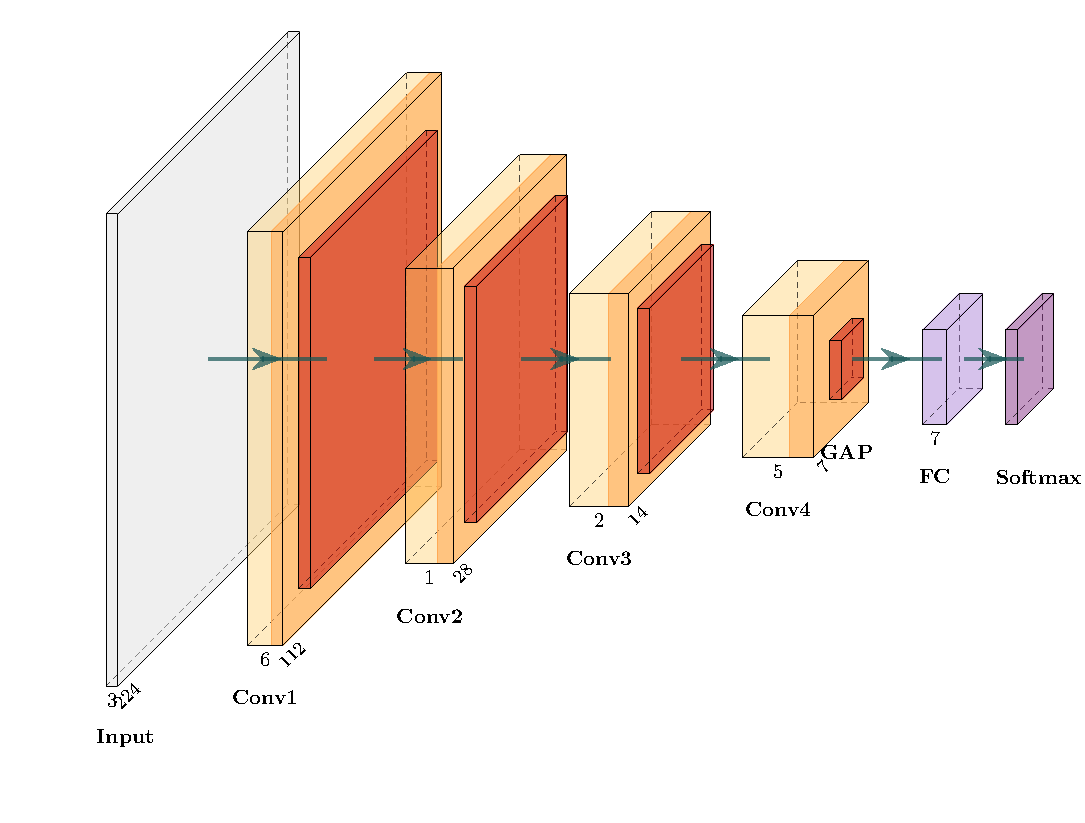
\includegraphics[width=\columnwidth]{figures/simplecnn.pdf}
\caption{SimpleCNN architecture: 4-block VGG-style network trained from scratch.}
\label{fig:simplecnn}
\end{figure}

\subsection{ResNet50}

ResNet50~\cite{He2016} with ImageNet-pretrained weights (\fig{fig:resnet50}). The original classifier is replaced by a two-layer head (2048$\rightarrow$512$\rightarrow$75) with dropout at 0.5 and 0.3, for 24.6M parameters in total. All layers are trainable.

\begin{figure}[ht]
\centering
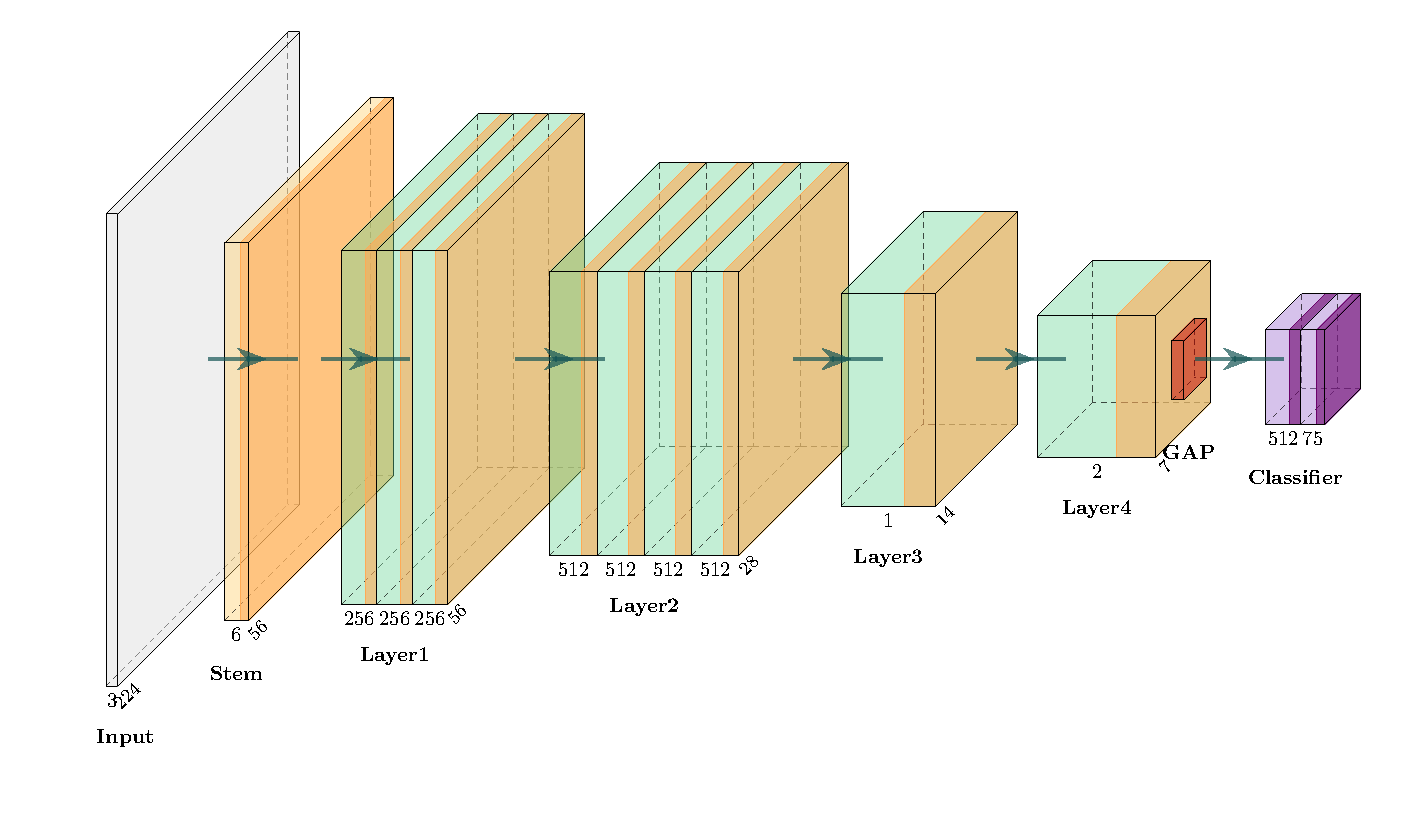
\includegraphics[width=\columnwidth]{figures/resnet50.pdf}
\caption{ResNet50 architecture with custom classifier head.}
\label{fig:resnet50}
\end{figure}

\subsection{EfficientNet-B0}

EfficientNet-B0~\cite{Tan2019} uses compound scaling over depth, width, and resolution (\fig{fig:efficientnet}). It is built from MBConv blocks with depthwise separable convolutions, Swish activations, and squeeze-and-excitation attention already inside each block. With a single dropout plus linear head it holds 4.1M parameters, 6$\times$ fewer than ResNet50.

\begin{figure}[ht]
\centering
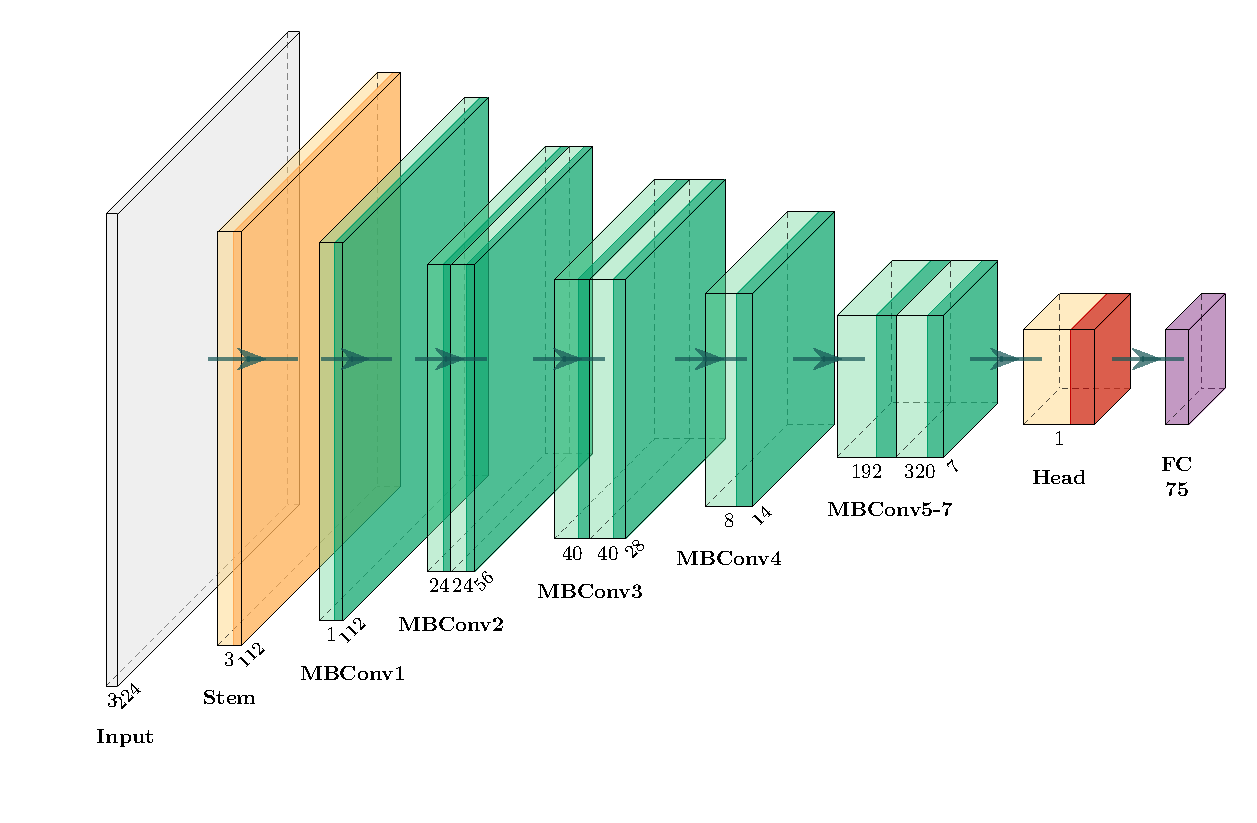
\includegraphics[width=\columnwidth]{figures/efficientnet.pdf}
\caption{EfficientNet-B0 architecture with MBConv blocks and SE attention.}
\label{fig:efficientnet}
\end{figure}

\subsection{ResNet50 with SE Attention}

ResNet50-SE inserts a Squeeze-and-Excitation block after each of the four residual stages (\fig{fig:resnet50se}). Each block performs global average pooling to squeeze the spatial dimensions, two fully-connected layers with reduction ratio 16 to model channel dependence, and sigmoid-gated rescaling of the original features. The four blocks add roughly 0.7M parameters (8K, 32K, 131K, and 524K for the 256, 512, 1024, and 2048 channel stages). The head is a single dropout plus linear layer, which is why the total (24.36M) sits slightly below the two-layer-head ResNet50 (24.60M) despite the extra attention parameters.

\begin{figure}[ht]
\centering
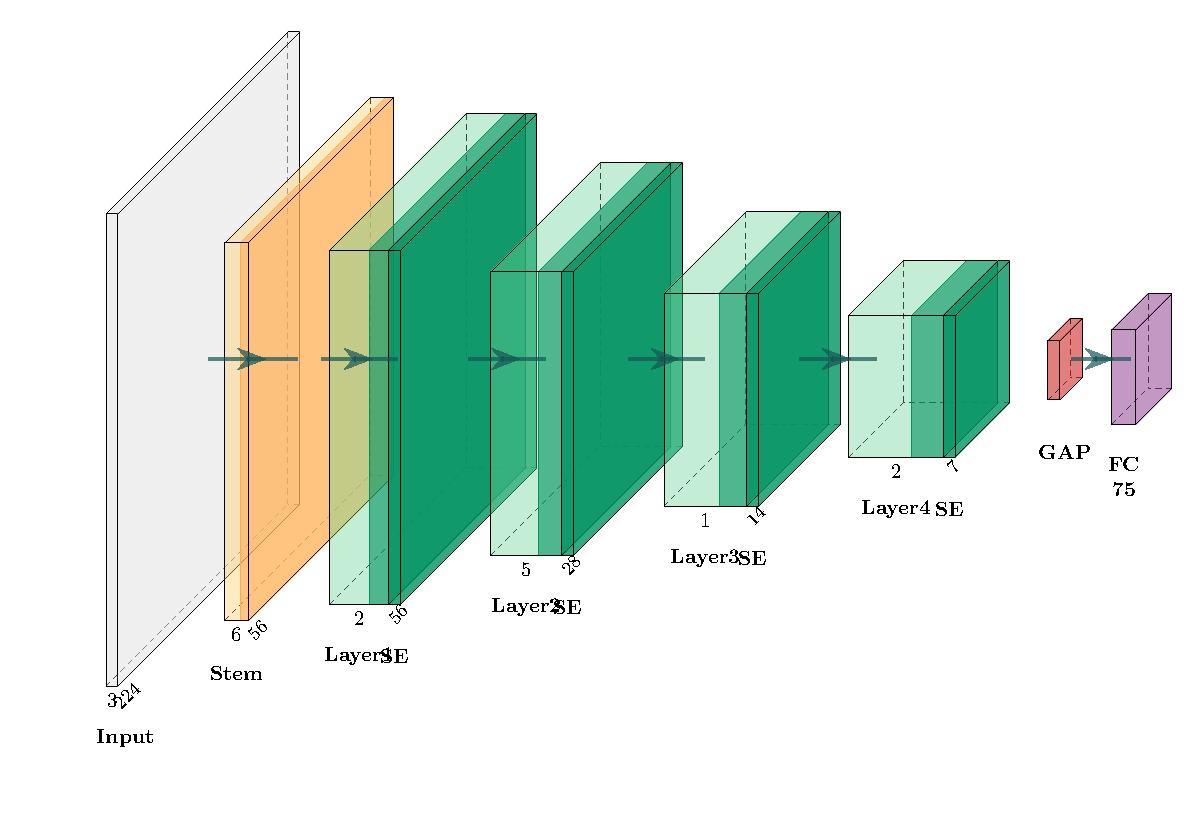
\includegraphics[width=\columnwidth]{figures/resnet50_se.pdf}
\caption{ResNet50-SE architecture with SE attention blocks after each stage.}
\label{fig:resnet50se}
\end{figure}

\subsection{Hierarchical Multi-Task Classifier}

The hierarchical classifier exploits the coarse-to-fine structure of the annotation (\fig{fig:hierarchical}). A shared ResNet50 backbone feeds two parallel two-layer heads: make (2048$\rightarrow$512$\rightarrow$75) and model (2048$\rightarrow$512$\rightarrow$431). Both heads see the same 2048-dimensional pooled feature. The auxiliary model task forces the backbone to retain the fine detail that separates variants inside a make, which the make head then reuses. Total parameters: 25.9M (23.5M backbone, 1.09M make head, 1.27M model head).

\begin{figure}[ht]
\centering
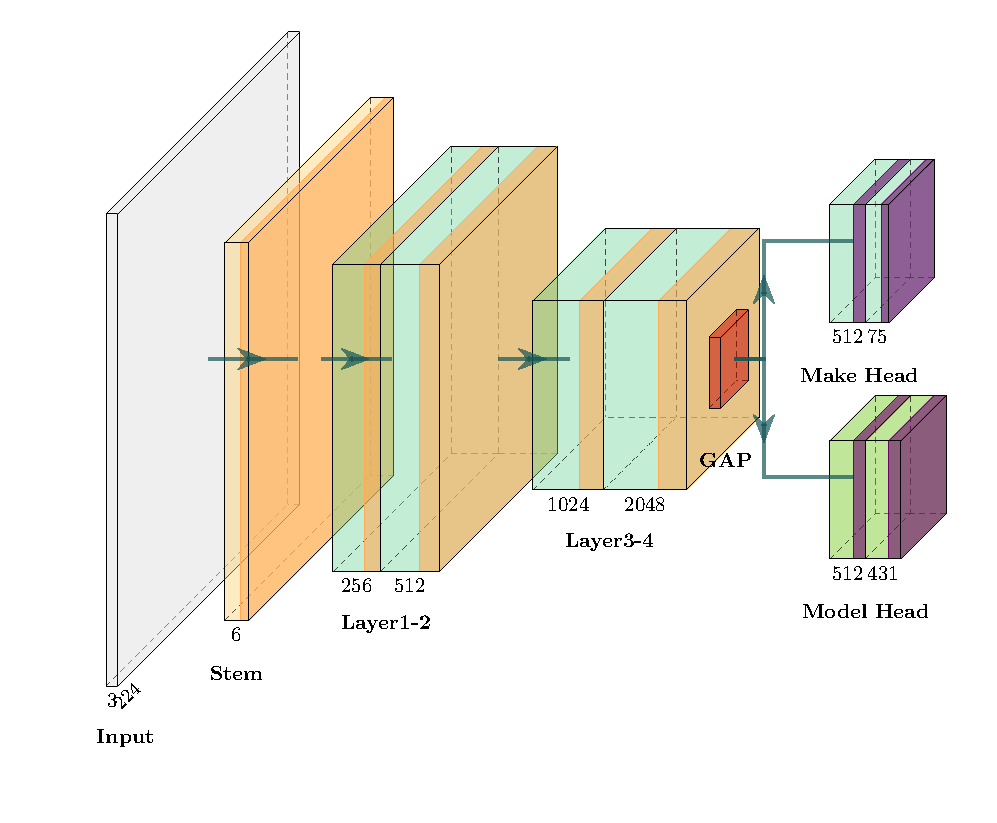
\includegraphics[width=\columnwidth]{figures/hierarchical.pdf}
\caption{Hierarchical classifier with shared backbone and dual classification heads.}
\label{fig:hierarchical}
\end{figure}

\section{Training Methodology}
\label{sec:learning_framework}

\subsection{Loss Functions}

\textbf{Cross-entropy.} The baseline. All misclassifications weighted equally regardless of class frequency.

\textbf{Focal loss.} Focal loss~\cite{Lin2017} with $\gamma$=2 down-weights easy examples so that gradient mass concentrates on hard ones. It is the standard answer to class imbalance and is included precisely to test that claim on this dataset.

\textbf{Label smoothing.} Cross-entropy with smoothing 0.1, which spreads a small probability mass over non-target classes and penalizes overconfidence.

\textbf{Hierarchical loss.} The multi-task model minimizes
\begin{equation}
\mathcal{L} = \alpha \cdot \mathcal{L}_{\text{make}} + (1-\alpha) \cdot \mathcal{L}_{\text{model}},
\label{eq:hier}
\end{equation}
with $\alpha$=0.3, so 70\% of the loss weight sits on the harder 431-class model task. Both terms use cross-entropy with label smoothing 0.1.

\subsection{Optimization Strategy}

AdamW with differential learning rates: $10^{-4}$ for pretrained backbones and $10^{-3}$ for the randomly initialized heads. The backbone keeps its ImageNet features while the heads adapt quickly.

Training ran for 100 epochs at batch size 32, weight decay $10^{-4}$, and gradient clipping at max norm 1.0. A ReduceLROnPlateau scheduler halved the learning rate after 3 epochs without validation improvement; early stopping with patience 5 restored the best validation checkpoint. Mixed precision (AMP) cut memory use by roughly 40\% on the 12GB RTX 3060 used for all runs. For the hierarchical model the scheduler and early stopping track make accuracy.

\subsection{Hyperparameter Summary}

\tab{tab:hyperparams} lists the configuration, identical across all experiments except for the loss.

\begin{table}[ht]
\centering
\caption{Training Hyperparameters}
\label{tab:hyperparams}
\begin{tabular}{ll}
\toprule
\textbf{Parameter} & \textbf{Value} \\
\midrule
Batch size & 32 \\
Backbone learning rate & $10^{-4}$ \\
Classifier learning rate & $10^{-3}$ \\
Weight decay & $10^{-4}$ \\
Epochs & 100 \\
Scheduler patience & 3 \\
Early stopping patience & 5 \\
Label smoothing & 0.1 \\
Hierarchical $\alpha$ & 0.3 \\
\bottomrule
\end{tabular}
\end{table}
